\documentclass[a4paper,11pt]{report}
\title{DeepDepth \\ An Approach To Visualize Twitter Tweets}
\author{AmirSaber Sharifi}
\date{October 2014}
\pagestyle{headings}

\usepackage{listings}
\usepackage{color}

\definecolor{dkgreen}{rgb}{0,0.6,0}
\definecolor{gray}{rgb}{0.5,0.5,0.5}
\definecolor{mauve}{rgb}{0.58,0,0.82}

\lstset{frame=tb,
  language=Java,
  aboveskip=3mm,
  belowskip=3mm,
  showstringspaces=false,
  columns=flexible,
  basicstyle={\small\ttfamily},
  numbers=none,
  numberstyle=\tiny\color{gray},
  keywordstyle=\color{blue},
  commentstyle=\color{dkgreen},
  stringstyle=\color{mauve},
  breaklines=true,
  breakatwhitespace=true
  tabsize=3
}

\usepackage{graphicx}
\graphicspath{ {./images/} }

\begin{document}

\maketitle

\tableofcontents

\chapter{Introduction}

\section{Social Network}

\subsection{What Is a Social Network}

These days we hear these words a lot, \emph{Social Network}. But what is a social network? According to \emph{Wikipedia} social network is:

\begin{quote}

A social network is a social structure made up of a set of social actors (such as individuals or organizations) and a set of the dyadic ties between these actors
\footnote{http://en.wikipedia.org/wiki/Social\_network/}.

\end{quote}

This definition may not seems familiar to us. If you ask people about definition of social network, you properly will hear answers like Facebook, Google plus, Twitter and etc. A more rational definition of social network is:

\begin{quote}

a dedicated website or other application that enables users to communicate with each other by posting information, comments, messages, images, etc.\footnote{Google result for query "What is social network?"}

\end{quote}

which is a more common definition between people these days.

As it can be seen in both definitions, social actors are key part of a social network. Individuals, organizations, governments and departments are playing the most important rule in a social network. Thanks to Internet, having access to variety of social networks made easy using desktops PCs and smart phones. People can be in contact almost anywhere in the world as long as they have any type of Internet connection such as cable, wireless, 4G and so on.

\subsection{Importance of Social Networks}

In 21st century data becomes one of the most important factor in analysis. Companies need data to do analysis and the more data they get the more assurance of accurate results they will have. Companies ask analysis experts to do various analytics tasks like number of customers, customers satisfaction and advertisement success. In most of these tasks people are playing a part. People may fill surveys on paper or online to participate in data analytic. But sometimes it's hard or expensive for companies to reach their considered group of people and even worse, those people don't feel like to participate or fill those long surveys forms.

Social networks are a rich resource of people opinions. People post, share and talk about different subjects in social networks. They may talk about something they like or about something they don't like. One company can gather most of the data they want just by looking at people posts. They can fetch and analyze users check ins, locations, hash tags and so many other useful information.

According to Facebook, there are 1,310,000,000 number of monthly active users on Facebook and 1 million links, 2 million friend requests and 3 million messages are sent through Facebook every 20 minutes
\footnote{http://www.statisticbrain.com/facebook-statistics/}.
Other social networks have amazing numbers also, like Twitter. There are  	645,750,000 active registered users on Twitter and their tweets will reach 58 million each day
\footnote{http://www.statisticbrain.com/twitter-statistics/}.
Considering these numbers there is no doubt that social networks should be a consideration to analyzers.

It's not only about companies. They are many other cases that social network's data may help. Like detecting spread of an epidemic disease based on people talking about special symptoms or predicting presidential elections. So many different usages can be found for social networks data and those examples can really show us how important is a social network and how it can help us.

\section{Twitter}

Twitter, started at 2006 is a micro blogging social network that allows users to post a message in 140 characters. Users can post and read twitter but unregistered users can only read tweets. Tweets can be posted using their web site, mobile apps or text messages.

\subsection{Statistics}

In Twitter there are about 1 million users and everyday about 500 million tweets are posted into Twitter. This huge number of data made me feel that Twitter is a good resource for gathering data.

\section{Data Analysis}

There are different analysis that can be made. One will look for analysis based on location or time. More complex analysis could be considered also. The thing that is important is to have a layer architecture so in one layer storing data would be done and in other layers analytics could be take place. With this approach adding more analysis to application will be easier.

\subsection{Visualizing Data}

After doing analysis visualization is important. Analysis with appropriate visualization will be a good resource for reasonings. It should be kept in mind in different analysis different visualizations are needed. To conquer this another layer would be considered which is the visualization layer. I, as the programmer, am able to make different visualization for different analysis and just link them. So user is able to see different graphs, charts or maps based on the analysis he requested.

\section{DeppDepth}

DeepDepth is the name of my application that do the tasks I mentioned. It's made of two side, client side and server side. In server side it will retrieve data from Twitter and save them into a database. After receiving user requests it will run analysis and make a result data. On client side, user can submit choose from different queries and type a keyword and submit his request. This request will be parsed into a query for database and after the result is ready user can see the result in different visualizations.

\chapter{Motivation}

\chapter{Background}
About background

\section{Related Works}
About related works


\section{Tools}

In this chapter I will describe what are the tools that I am using to implement my project. Some of these tools are used in client side and some of others are used in server side. I will briefly describe each tool and tell how I used that.

\subsection{Twitter APIs}

Twitter provide APIs for accessing tweets posted by users. These data are not all the tweets but they are samples of them. To get all the data one needs to be Twitter partner so he can access to all Twitter tweets. Twitter APIs are mainly Search API and Streaming API. I choose Streaming API over Search API. Here you can see the differences and why I choose Streaming API.

\subsubsection{Search API}

By going to developer center in Twitter web site users can start making applications for Twitter and use on of the APIs. Search API is a RESTful API that accept queries from application and send back the result in JSON. Applications using this search query can have filters like a hash tag, a specific keyword, location or time. Using this API is a good practice but there are some limitations. Rate limits are divided into 15 minutes window and in each of them only 180 queries can be made. I was visioning to use this API at the begging and by having fake users overcome the limitation that I received a notice about abusing their service and I asked to stop this. So I was forced to switch to Streaming API which does not have any limitation. 

\subsubsection{Streaming API}

In Streaming API, application will receive tweets that are posted from now on. There are 3 endpoint for using this API: Firehose, Sample and Filter.

\emph{Firehose} will send all and every single tweet posted in Twitter and it needs to be Twitter partner to access it.

\emph{Sample} will stream only 1 percent of all tweets to application. It's a good endpoint for applications that want to look at data around the world and run some tests.

\emph{Filter} is the endpoint I'm using for my application. With this endpoint you can filter sample endpoint data using some filters like location, language or keyword. In my project I used filter based on location which topoJson boundary of united states. Figure \ref{fig:hbcus} shows the bounding coordinates I am using.

\begin{figure}[!hbp]
\caption{Location of united states in HBC}
\begin{lstlisting}
// United states coordinate in Java
Location unitedStates = new Location(new Coordinate(-125, 30), new Coordinate(-60, 50));
\end{lstlisting}
\label{fig:hbcus}
\end{figure}

\subsubsection{HBC}
For using any of APIs there should be a client application that connect to that API. To do so there are some libraries for different languages. HBC, Hosebird Client, is the official Twitter library written in Java. I am using this library to connect to API and receive tweets from United States. In figure \ref{fig:hbccode} you can see the most important part of the code I've written.

\begin{figure}[!hbp]
\begin{lstlisting}
BlockingQueue<String> queue = new LinkedBlockingQueue<String>(10000);
// Create Locations
Location unitedStates = new Location(new Coordinate(-125, 30),new Coordinate(-60, 50));

// Define our endpoint: By default, delimited=length is set (we need
// this for our processor)
// and stall warnings are on.
StatusesSampleEndpoint endpoint = new StatusesSampleEndpoint();
StatusesFilterEndpoint filterEndPoint = new StatusesFilterEndpoint();
filterEndPoint.locations(Lists.newArrayList(unitedStates));
filterEndPoint.stallWarnings(true);
endpoint.stallWarnings(false);

Authentication auth = new OAuth1(consumerKey, consumerSecret, token,secret);

// Create a new BasicClient. By default gzip is enabled.
BasicClient client = new ClientBuilder().name("TwitterCrawler").hosts(Constants.STREAM_HOST)
	.endpoint(filterEndPoint)
	.authentication(auth)
	.processor(newStringDelimitedProcessor(queue))
	.build();
/ Establish a connection
client.connect();
// Do whatever needs to be done with messages
while (true) {
	if (client.isDone()) {
    	System.out.println("Client connection closed unexpectedly: "
    	client.getExitEvent().getMessage());
    	break;
    }
	String msg = queue.poll(5, TimeUnit.SECONDS);
	if (msg == null) {
		System.out.println("Did not receive a message in 5 seconds\n");
	} else {
		if (msg.indexOf("\"country_code\":\"US\",") > -1) {
			System.out.println("@[" + databaseName + "." + tableName + "] " + msg);
		}
	}
}
\end{lstlisting}
\caption{Using HBC to recieve Data}
\label{fig:hbccode}
\end{figure}

\subsection{Big Data}

Number of tweets posted in Twitter in United States that my application receive is millions. Thus storing them and analyzing them needs an special approach to do it fast and efficient. MapReduce is a great idea to do so. By using MapReduce each analyze task can be divided into chunks specially when analyses are based on date.

\subsubsection{Hadoop}

Hadoop is on open source implementation of MapReduce made by \emph{Apache}. It let us to run MapReduce jobs on big files on "HDFS". So it's needed to store tweets into HDFS after receiving them. Here was my next challenge. How to store them in HDFS. Tweets could be written directly into HDFS using some tools or even directly. But I found another solution which is more flexible and can help the project even in defining Map Reduce Jobs which is Hive.

\subsubsection{Hive}

Based on Hive web page Hive is:
\begin{quote}
The Apache Hive ™ data warehouse software facilitates querying and managing large datasets residing in distributed storage. Hive provides a mechanism to project structure onto this data and query the data using a SQL-like language called HiveQL. At the same time this language also allows traditional map/reduce programmers to plug in their custom mappers and reducers when it is inconvenient or inefficient to express this logic in HiveQL.
\end{quote}
After installing Hive on a computer, Hive will connect to HDFS and store it's database there. Thus user would be able to define queries for Hive so that Hive will make it a MapReduce job and run it on Hadoop and send back the result in different formats like JSON, CSV or etc.

\subsubsection{HiveQL}

Hive uses a SQL like language for making MapReduce jobs and run them. One example of this HiveQL which creates a table in database is show in figure \ref{fig:hiveqltable}.

\begin{figure}[!hbp]
\caption{HiveQL example for creating a table and partitioning that table}
\begin{lstlisting}
CREATE TABLE invites (foo INT, bar STRING) PARTITIONED BY (ds STRING);
\end{lstlisting}
\label{fig:hiveqltable}
\end{figure}

Figure \ref{fig:hiveqlwordcount} shows an example of word count query in HiveQL. As it can be seen it receive all words and count each of them as one and then group them. So the result will be a table of word and number of occurrence for that word.

\begin{figure}[!hbp]
\caption{HiveQL Word Count Example}
\begin{lstlisting}
SELECT word, COUNT(*) FROM input LATERAL VIEW explode(split(text, ' ')) lTable as word GROUP BY word;
\end{lstlisting}
\label{fig:hiveqlwordcount}
\end{figure}

HiveQL can be used in different ways to do our required analytics. For example in my project I need to get tweets with a special keyword in it and group them by location and count them. Figure \ref{fig:hiveqltweet} shows an example of getting result for keyword "New Mexico".

\begin{figure}[!hbp]
\caption{An example of query used in the project}
\begin{lstlisting}
SELECT get_json_object(tweets_us.place,'$.full_name') AS name, get_json_object(tweets_us.place,'$.bounding_box') AS coordinates, COUNT(1) AS cnt FROM tweets_us WHERE v['text'] LIKE '%New Mexico%' GROUP BY get_json_object(tweets_us.place,'$.full_name'), get_json_object(tweets_us.place,'$.bounding_box') ORDER BY cnt DESC
\end{lstlisting}
\label{fig:hiveqltweet}
\end{figure}

\subsubsection{Pig}

Hive also supports Pig. Based on Pig web page pig is:
\begin{quote}
Apache Pig is a platform for analyzing large data sets. Pig's language, Pig Latin, is a simple query algebra that lets you express data transformations such as merging data sets, filtering them, and applying functions to records or groups of records. Users can create their own functions to do special-purpose processing.
\end{quote}

Figure \ref{fig:hiveqlpig}  demonstrates Word Count example written in Pig. In this example it loads a file and then for each line it separate that line with spaces and considering each part as a word it counts them.

\begin{figure}[!hbp]
\caption{Pig Word Count Example}
\begin{lstlisting}
A = load './input.txt';
B = foreach A generate flatten(TOKENIZE((chararray)$0)) as word;
C = group B by word;
D = foreach C generate COUNT(B), group;
store D into './wordcount';
\end{lstlisting}
\label{fig:hiveqlpig}
\end{figure}

\subsection{JavaScript}

JavaScript used to be a hated language but now is fast growing programming language because of unifying client side and server side programming languages. By using Javascript and it's different frameworks programmer will be able to write it's client side and server side in the same language and by using JSON interaction of client and server made really easy. That's why in my project I used Javascript as the programming language.

\subsubsection{NodeJs}

Google release a Javascript runtime engine which name is V8. NodeJs is a platform using that engine to run JavaScript as an application on server side. It's scalable and making network application are made really easy using some features of NodeJs. By using NodeJS I make a web server that host my application which is written in JavaScript and using some other frameworks that I will describe them later. Figure \ref{fig:nodejsserver} shows a simple web server that returns "Hello World" to every request.

\begin{figure}[!hbp]
\caption{Simple NodeJS Web Server}
\begin{lstlisting}
var http = require('http');
http.createServer(function (req, res) {
  res.writeHead(200, {'Content-Type': 'text/plain'});
  res.end('Hello World\n');
}).listen(1337, '127.0.0.1');
console.log('Server running at http://127.0.0.1:1337/');
\end{lstlisting}
\label{fig:nodejsserver}
\end{figure}

\subsubsection{MongoDB}

As most web applications needs a database to work with I choose MongoDB. It's a light weighted , documented oriented database. I found this database appropriate to my project because of it's Json like documents support.

\subsubsection{ExpressJS}

Express is a web application framework written in NodeJS. Since I am using NodeJS and Javascript I found this framework easy to work with. It supports HTTP and HTTPS request and by using middlewares it makes it easy to handle HTTP requests. Implementing security and logging features is done using Passport which is another NodeJS module.

\subsubsection{AngularJs}

For general controllers I used AngularJs which is a client side script that is really good for updating the page without refreshing the whole entire page. I used this for controllers like registering user or submitting a query and get result of a job processed by Hive.

\subsubsection{D3Js}

The next and final tool in our tool key chain is the visualizer. D3Js is a library that is able to create different kind of charts and graphs using Javascript on browsers. By using AngularJs, I receive result of a job from the database and then send it to D3Js to plot it. In project there different kind of plotters that the project will choose one based on the data and the visualization that user choose. Figure \ref{fig:d3usanewmexico} shows a result of query looking for keyword "Ebola" in D3Js

\begin{figure}[!hbp]
\begin{center}
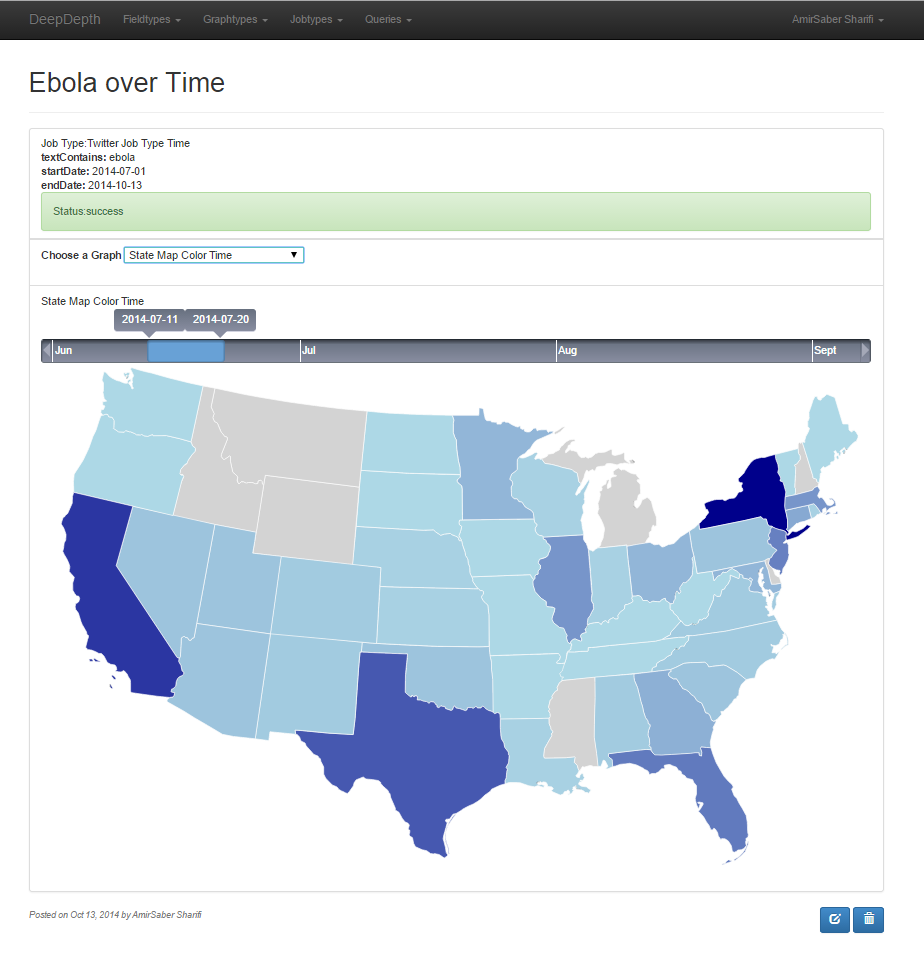
\includegraphics[scale=0.5]{map.png}
\end{center}
\caption{Map of united states based on number of people twitting about Ebola between 11-07-14 to 28-07-2014}
\label{fig:d3usanewmexico}
\end{figure}

\chapter{DeepDepth}

About Deepdepth

\section{Server}

About Server

\subsection{Config}

About Configs

\subsection{Models}

About Models

\subsection{Controllers}

About Controllers

\subsection{Routes}

About Routes

\subsection{Tasks}

About Tasks

\subsection{Tests}

About Tests

\subsection{Views}

About Views

\section{Client}

About Client

\subsection{Modules}

About Modules

\subsubsection{config}

About configs

\subsubsection{Controllers}

About Controllers

\subsubsection{Services}

About Services

\subsubsection{Views}

About Views

\subsubsection{Tests}

About Tests

\section{Users}

User types

\subsection{Admin}

About admin and admin tasks

\subsection{Users}

About user and user tasks

\chapter{Difficulties}

In the initial project plan there were some ideas that changed during project coding. I try to mention them and tell why that happened.

\section{Gathering data}

At the begging I was visioning to use Search API of Twitter and by using ZooKeeper, I can have different users to attack limitation of API. But because of the notice I changed my plan to using Streaming API and by using Streaming API there is no reason to use ZooKeeper.

The other problem is because of using Filter endpoint my application is not receiving all tweets in united states. I couldn't do any thing about it because of Twitter policy.

Streaming API needs an always on client to receive the data and store them in database, this was the other problem that I faced so I used Heroku cloud platform to solve this issue.

\section{Computation}

I received about 2 million tweets each day, storing them and doing analysis on them was another difficulty that I faced. It needs a lot of storage space and processor power. I tackled this issue by using TreasureData cloud storage which implements Hive to store the database.

\section{Visualization}

For every different type of query there should be a new type visualization. By using layer architecture I tried to conquer it as much as possible but making a visualization takes a long time to program and validate. So for each new query or visualization I want to add to project it will need lots of effort.

\chapter{Implementation}

As mentioned before an always running machine with lots of storage space and processing power is needed to do this project. Thus I decided to used cloud platforms, the most convenient one I found for my project is Heroku which is also a semi free service.

\section{Heroku}

Heroku is a cloud platform that sand it's made of a worker and a web and supports different languages like Java, PHP, NodeJS and etc. Each program with be packaged as a sand box named Dyno. These Dynos can be any type of Worker or Web or both. Workers are softwares that don't have a web interface. Since in free service there can be only a worker or a web I just made a worker to retrieve tweets from Twitter Streaming API and save them into the database. In Heroku you can have plug ins. Plug ins are third party services that can be used for the application. For storing my data into a Hive database I used TreasureData.

\section{TreasureData}

Having a large database in Hive and running MapReduce jobs on it needs resources. I ended up using TreasureData cloud service to store my tweets into it. They provide 150GB of storage and some compression algorithm to reduce size of data. By \today I saved 50 million tweets. After saving tweets into Hive database by using TreasureData API HiveQL queries can be send to TreasureData server and it will compute the result and response in requested format. Figure \ref{fig:tddetail} shows a detail of job executed on Treasure Data.

\begin{figure}[!hbp]
\caption{Treasure Data detail of a job}
\begin{lstlisting}
Total MapReduce jobs = 2
Launching Job 1 out of 2
Number of reduce tasks not specified. Defaulting to jobconf value of: 4
In order to change the average load for a reducer (in bytes):
  set hive.exec.reducers.bytes.per.reducer=<number>
In order to limit the maximum number of reducers:
  set hive.exec.reducers.max=<number>
In order to set a constant number of reducers:
  set mapred.reduce.tasks=<number>
Starting Job = job_201306191947_855672, Tracking URL = http://ip-10-149-50-132.ec2.internal:50030/jobdetails.jsp?jobid=job_201306191947_855672
Kill Command = /usr/lib/hadoop/bin/hadoop job  -kill job_201306191947_855672
Hadoop job information for Stage-1: number of mappers: 4; number of reducers: 4
2014-04-22 16:40:37,607 Stage-1 map = 0%,  reduce = 0%
2014-04-22 16:40:46,722 Stage-1 map = 3%,  reduce = 0%
....
....
\end{lstlisting}
\label{fig:tddetail}
\end{figure}

After the job is finished it will return result of the job in Hive supported formats such as JSON and CSV. Figure \ref{fig:tdcsv} shows abbreviated some rows of a csv file as a result of job in Treasure Data.

\begin{figure}[!hbp]
\caption{Treasure Data CSV result of a job}
\begin{lstlisting}
name,coordinates,cnt
"Albuquerque, NM","{""type"":""Polygon"",""coordinates"":[[[-10,34],[-106,35],[-106,35],[-106,34]]]}",72
"New Mexico, USA","{""type"":""Polygon"",""coordinates""....}",54
"Texas, USA","{""type"":""Polygon"",""coordinates""....}",15
"Arizona, USA","{""type"":""Polygon"",""coordinates""....}",13
Rio Rancho,"{""type"":""Polygon"",""coordinates""....}",11
"Santa Fe, NM","{""type"":""Polygon"",""coordinates""....}",9
"Las Cruces, NM","{""type"":""Polygon"",""coordinates""....}",7
"University Park, NM","{""type"":""Polygon"",""coordinates""....}",6
\end{lstlisting}
\label{fig:tdcsv}
\end{figure}

\chapter{Summery}

As a result of this project, I was able to visualize Twitter tweets and get some meaningful data. Like seeing places where people talk about an special topic more. In the queries I tested like "New Mexico" the data makes sense. As It could be seen in Figure \ref{fig:d3usanewmexico} people who are talking about "New Mexico" are located mostly in New Mexico.

\section{Future works}

There are a lot to be improved in this project. I will mention some of them that I'm visioning to do in future.

\subsection{Other Social Networks}

My project works on Twitter tweets as it's data and only source. It will be great to be able to crawl into other social network data and let the user to choose which social network he wants to be analyzed or even choose a combination of them.

\subsection{Real Time}

Every time user submit a query he should wait for the result. It would be great to come up with an approach that compute the result in almost a real time manner. In that essence user can see the result just by waiting for seconds and even can scroll in time easily. Thus by having real time analysis other visualization can be made and it can improve the project a lot.

\subsection{Data Mining}

I am visioning to have a kind of data mining approach that by looking at frequent words in a query result try to guess what is that keyword and make a understanding of what people think about that special topic. Like as a restaurant owner by typing his restaurant name the code will find what people think about his restaurant, do they like it or not or even why do they like it.

\subsection{Data}

One problem is that I don't receive all the tweets. So my data set is not complete. In future this project can work with Twitter partners like GNIP to get access to all tweets and process on them. Maybe this project might be able to be a Twitter partner it self so it wouldn't need to pay to other companies to get access right to their data.

\listoffigures

\end{document}